\documentclass{article}


\usepackage[nottoc,numbib]{tocbibind}
\usepackage[utf8]{inputenc}
\usepackage{graphicx}
\usepackage{subcaption}
\usepackage{geometry}
\usepackage{amssymb}
\usepackage{caption}
\usepackage{float}
\usepackage{wrapfig}
\usepackage{romannum}
\usepackage{physics}
\usepackage{amsmath,amsfonts,amsthm,bm} % Math packages
\geometry{margin=1in}

\errorcontextlines 10000
\begin{document}
\pagenumbering{gobble}
\begin{titlepage}
    \begin{center}
        \vspace*{1cm}
        \Large

\includegraphics[width=.4\linewidth]{../logo.pdf}\\
        \Large
\vspace{1cm}
        Machine Learning Practicum\\
        \huge
        \textbf{Determining elasticity constants in nematic liquid crystal\\}
\Large  
        \vspace{1cm}
        \textbf{Andrej Kolar - Po{\v z}un\\}
        \vspace{0.8cm}

\vfill
\normalsize
\end{center}. 
\end{titlepage}
\newpage
\pagenumbering{arabic}
\section*{Intro}
This exercise deals with a useful aspect of soft matter physics liquid crystals - enlogated molecules, which have numerous applications, most notably in LCD (liquid crystal display) screens. In order to better understand this project it will be necessary to delve a bit more into the physics compared to the previous reports.

Different liquid crystals possess different deformation properties - these are determined by the elasticity constants $K_{11}, K_{22}, K_{33}$ that govern how the crystals will behave under different deformation types (splay, twist and bend, respectively). Naturally, knowing these constants is of great interest for industrial use.
This is usually expressed by (Frank) free energy density:
\begin{equation*}
f = \frac{1}{2} K_{11} \left( \nabla \cdot \vec{n} \right)^2 + \frac{1}{2} K_{22} \left( \vec{n} \cdot \nabla \times \vec{n} \right)^2 + \frac{1}{2} K_{33} \left( \vec{n} \times \nabla \times \vec{n} \right)^2,
\end{equation*}
where $\vec{n}$ is a spatially dependent director - a pseudovector giving the direction of the enlogated moleculess.



The usual procedure for determining these constants is to subject the liquid crystal to some electric field, which can be expressed by adding the following term to the free energy:
\begin{equation*}
f_e = - \frac{1}{2} \epsilon_0 \epsilon_a \left( \vec{n} \cdot \vec{E} \right)^2
\end{equation*}

This implies that changing the value (or direction) of the electric field with respect to $\vec{n}$ will have an effect on their structure. It turns out that indeed, if the liquid crystals are put between two plates at distance $d$, above a certain value of critical electric field $E_c$, the liquid crystals will orient themselves. The value of the critical electric field depends on the elastic constant in the following way:
\begin{equation*}
E_c = \frac{\pi}{d} \sqrt{\frac{K_i}{\epsilon_0 \epsilon_a}},
\end{equation*}

where $K_i$ is one of the elastic constants. It is possible to anchor the liquid crystals at the boundaries (the plates) to force only one of the three elastic constnts to be relevant at the time. The point where the crystals orient can be experimentally measured by either measuring the capacity of the system or measuring the intensity of light that passes through them.

This gives an experimental way of determining $E_c$ and hence the elastic constants of the crystal. However... This is notoriously hard - it is difficult to control all the aspects of the experiment precisely and even for the more commonly used liquid crystals the values of the elastic constants vary greatly.... In this project, we will try to develop an alternative approach to determine those constants.

\section*{An alternative approach of calculation}

For our approach, we will use the fact that is very much used in LCDs - the intensity of the electric field flowing through the crystals depends on their orientation. 
More precisely, they are anisotropic materials and the index of refraction of such a material is incident electric field angle dependent:
\begin{equation*}
\frac{1}{n(\theta)^2} = \frac{\cos^2 \theta}{n_e^2} + \frac{\sin^2 \theta}{n_o^2},
\end{equation*}
where $\theta$ is position dependent, as it is the relative angle between the incident wave and the liquid crystals (and we know that the direction of liquid crystals is position dependent).

The plan is as follows:
\begin{itemize}
\item Start with some initial configuration of the liquid crystal (can be obtained by a strong light pulse).
\item Shine a beam of light through the sample of our liquid crystal.
\item As it relaxes to its stationary state, the index of refraction will change over time.
\item This relaxation and therefore the index of refraction depend on material properties (elastic constants).
\item This will affect the intensity of light that comes through the sample and can easily be measured - $I(t)$.
\item Therefore we know the intensity of light is connected to the elastic constants but we do not know how.
\item We will train an artificial neural network to learn the connection.
\end{itemize}

So here comes the machine learning part - we will use a neural network to give us the elastic constants from our measurement of the intensity of light passing through the liquid crystal.

\section*{Preparing the data }

One thing everyone knows about neural networks is that they need alot of data to be trained. Data that we usually do not have. And in this case some kind of simulation or data augmentation must be employed. Since we really have no data, we will go with the former.

\subsection*{Theory}

Again our setup is liquid crystals between two plates. As mentioned, the direction of the liquid crystal is dependent on $z$ $\vec{n}(z)$. This in turns means that the previously mentioned index of refraction also depends on $z$ -  $n(z)$.
Without delving too much into the anisotropic materials theory, let us just mention that the incident light generally splits into two polarisations, which are affected by different indices of refraction. $n(z)$ and $n_o$, respectively.
The phase change after passing through the sample is given simply by 
\begin{equation*}
\Gamma = \frac{2 \pi}{\lambda} \int_0^d \left( n(z) - n_o \right) \textup{d}z
\end{equation*}

For our simulation we will simplify our life and assume the director field is given as:
\begin{equation*}
\vec{n}(z) = ( \cos \theta(z) , 0, \sin \theta(z) ).
\end{equation*}
Plugging into Frank energy we get:
\begin{equation*}
f = \frac{1}{2} K_{11} \left( \frac{\partial n_z}{\partial z} \right)^2 + \frac{1}{2} K_{33} \left( \frac{\partial n_x}{\partial z} \right)^2 
\end{equation*}

We will be interested about relaxation from some initial profile $\theta(z, t=0)$. This follows from the Frank energy by the Euler-Lagrange equations:
\begin{equation*}
\frac{\textup{d}}{\textup{d}z} \frac{\partial f}{\partial \theta^\prime} - \frac{\partial f}{\partial \theta} = \gamma_1 \frac{\partial \theta}{\partial t},
\end{equation*}
where the constant $\gamma_1$ is known in the experiment. The above E-L equation reduces to:
\begin{equation*}
\frac{\partial^2 \theta}{\partial z^2} (K_{11} \cos^2 \theta + K_{33} \sin^2 \theta ) + \frac{1}{2} (K_{33}-K_{11}) \left( \frac{\partial \theta}{\partial z } \right)^2 \sin 2 \theta = \gamma_1 \frac{\partial \theta}{\partial t}
\end{equation*}

For the case that $K_{11}=K_{33}=K$ (we will start with this simpler case) the above reduces to:
\begin{equation*}
\frac{K}{\gamma_1} \frac{\partial^2 \theta}{\partial z^2} = \frac{\partial \theta}{\partial t}
\end{equation*}

Having $\theta(z,t)$ and therefore also $n(z,t)$ and $\Gamma(t)$, we can derive $I(t)$ from geometric optics (Jones calculus). In our setup the incident wave is polarised linearly along $y=x$ line and after passing the crystal its polarisation along $y=-x$ line is measured. The intensity should behave as:
\begin{equation*}
I(t)  = \sin^2 (\Gamma(t)/2)
\end{equation*} 

\subsection*{Practice}
So to train a neural net, we need a huge number of elastic constants $K$, their intensity time evolutions $I(t)$ and initial configurations of liquid crystals $\theta(z,t=0)$.
We obtain these triples by simulation:
\begin{itemize}
\item First, uniformly sample a constant $K$ from the interval $K \in (0,K_\mathrm{max} = 20 pN)$.
\item Sample a smooth function $\theta(z)$ with given BC (for now, $\theta(0)=\theta(d) = 0$).
\item Solve the differential equation for $\theta(z,t)$.
\item Calculate $\Gamma(t)$ and in turn $I(t)$.
\end{itemize}

The way the initial function is sampled is as follows: Connect $(0,\theta(0))$ and $(d,\theta(d))$ linearly. Sample that function equidistantly. Randomly perturb each point to get a new function. Interpolate with a quadratic interpolant to get a smooth initial condition.

The differential equation that we are solving is a simple diffusion equation that we can solve in an explicit manner, while for $\Gamma(t)$ we can approximate the integral with a weighted sum. We will not delve into the specifics beyond that as they are more of a numerical analysis nature.

\subsection*{Example data}

Some example data can be seen on Figure \ref{fig:data}. In order to get even more data corresponding to a single elastic constant $K$, we can change the wavelength of the incoming light (affects $\Gamma(t)$).
The results for different $K$ and $\theta_0$ are very different and the relationship between the upper and middle/last row seems very nontrivial. The question is, will the neural network be able to learn this relationship well enough?

\begin{figure}[H]
\centering
\begin{subfigure}{.8\textwidth}
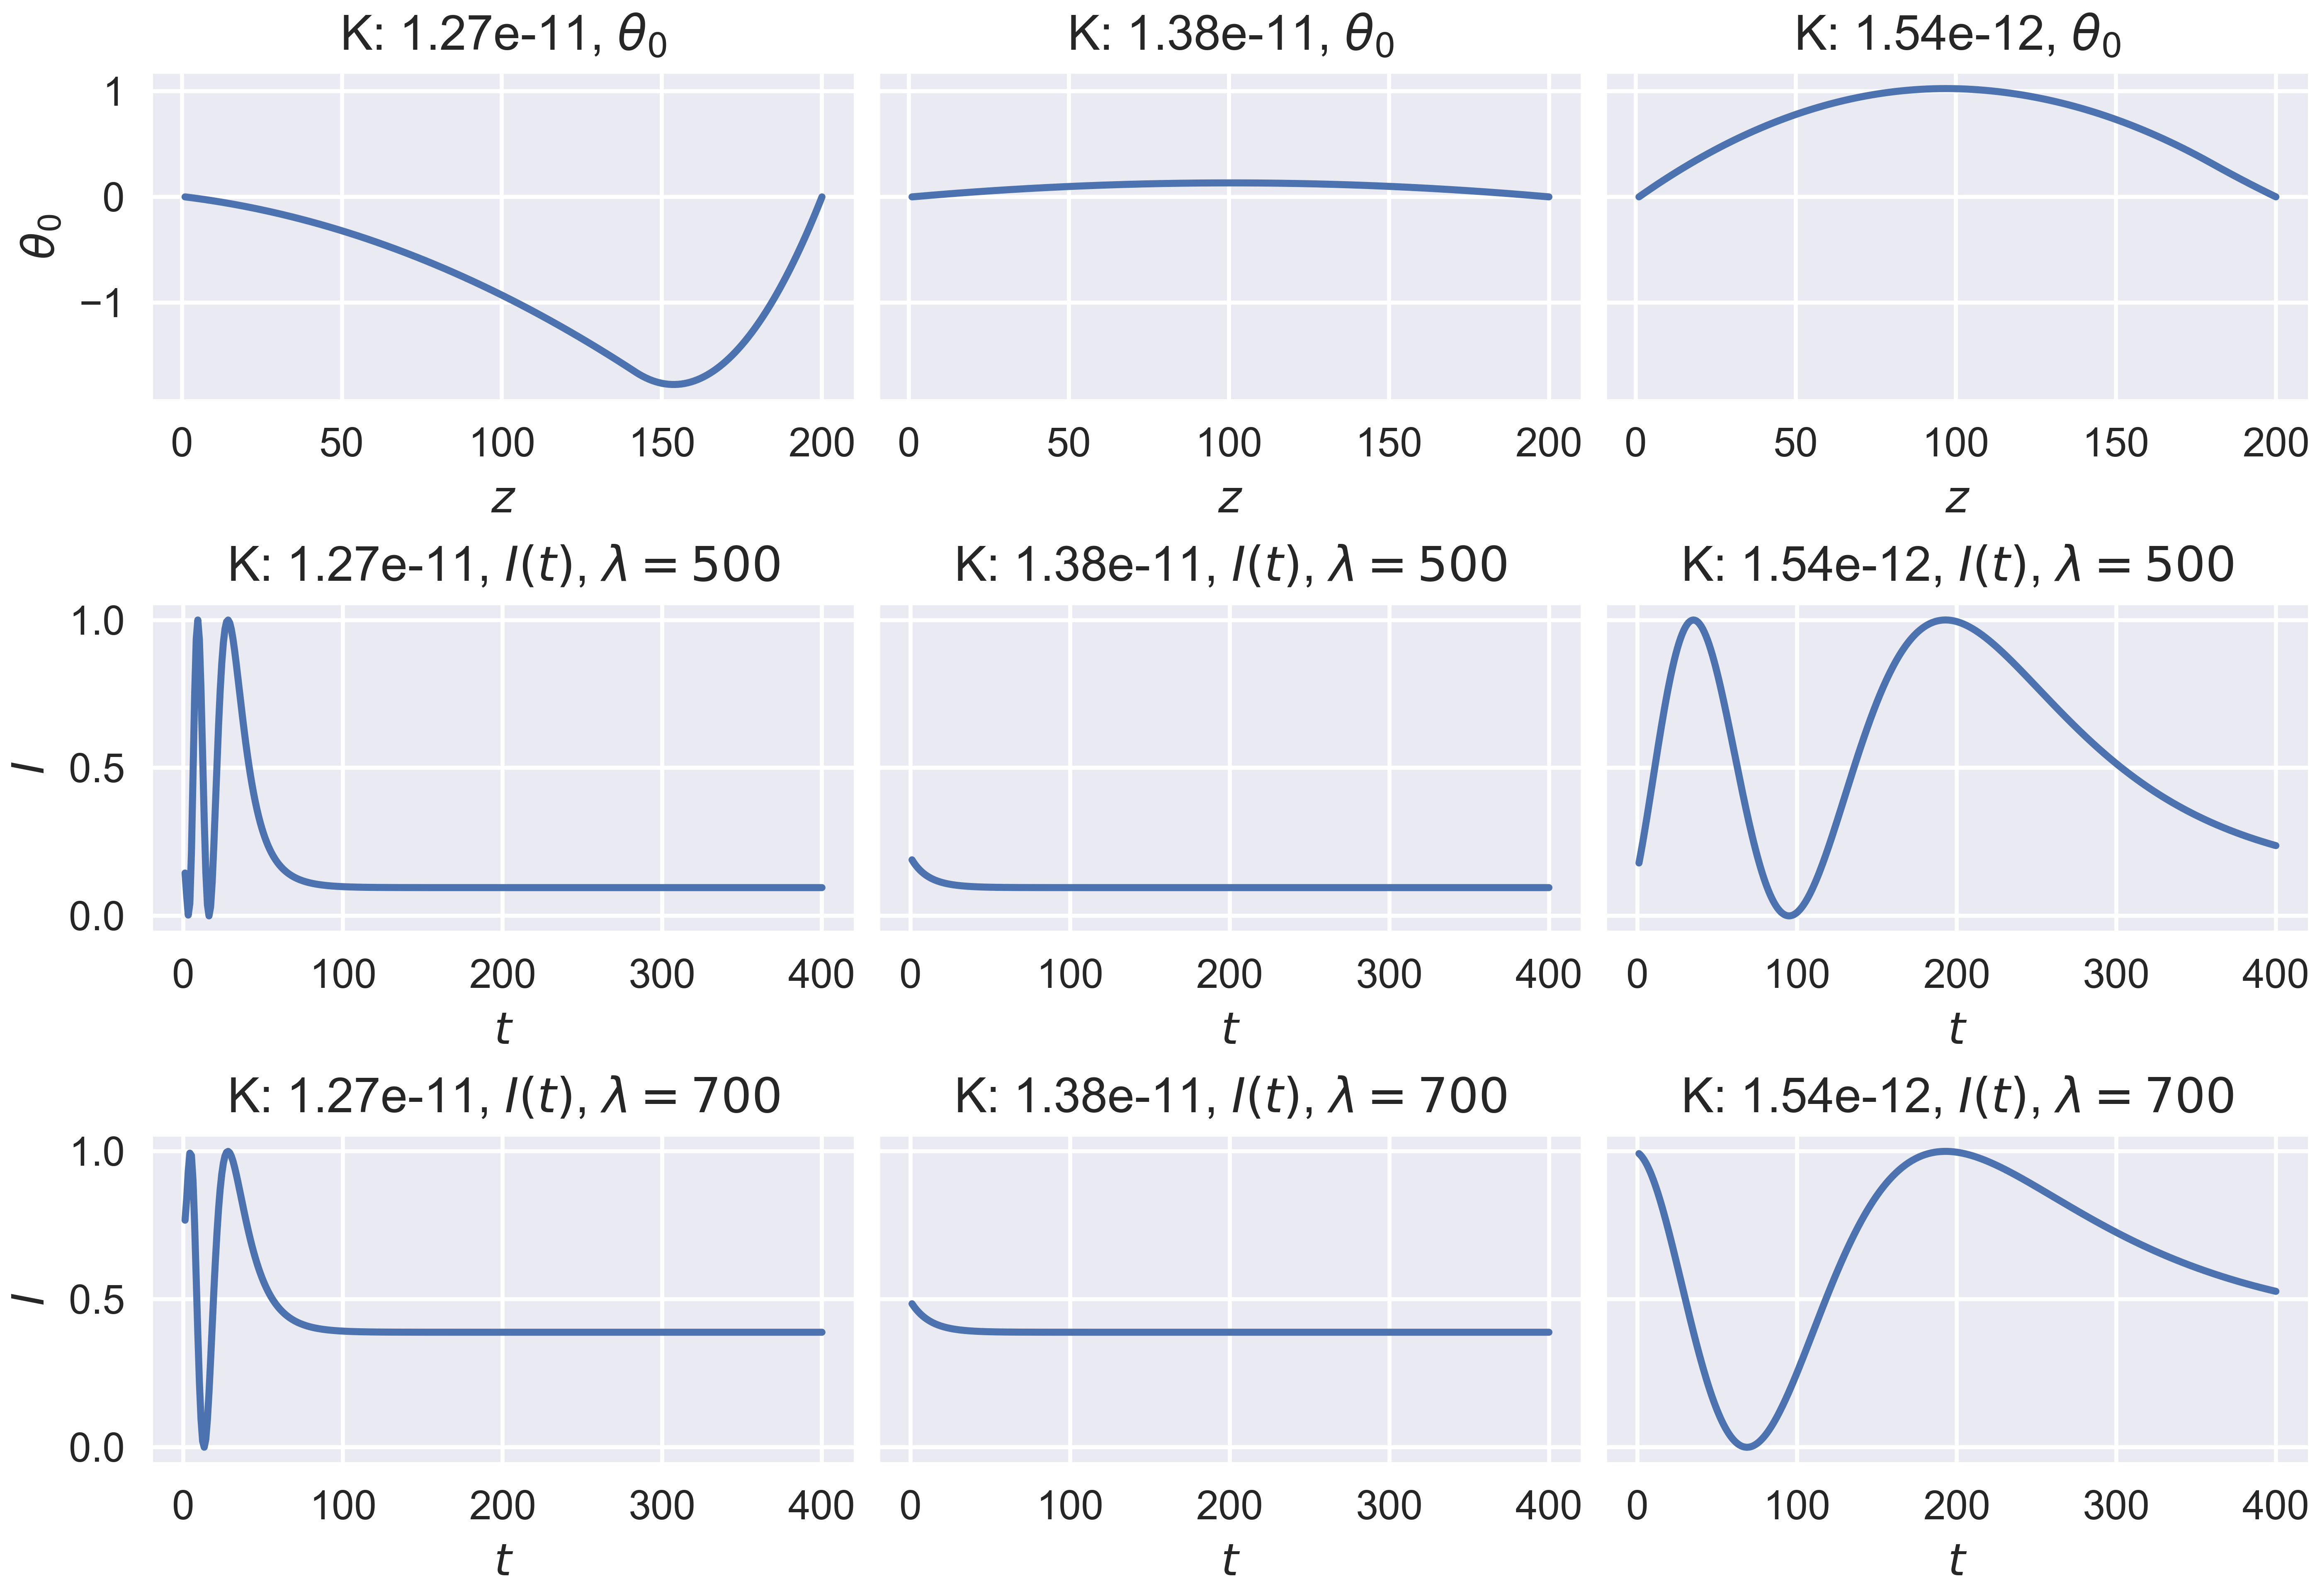
\includegraphics[width=\linewidth]{Figures/data.png}
\end{subfigure}
\caption{Each column corresponds to a different simulation (and different $K$). Top row: Initial profile $\theta_0(z)$. Second row: $I(t)$ result for $\lambda = 500$, third row: $I(t)$ for $\lambda=700$.}
\label{fig:data}
\end{figure}

\section*{Network structure}
We wil set up the network using Tensorflow (Keras) and we have generated ~500000 input/output pairs using the data preparation technique explained in the previous section.

First we split our data in the training and test set. I have opted to use 95\% of my data for training and the remaining 5\% for validation. The data was generated randomly so there is a (very) neglible probability that our training and validation sets would have data with very different characteristics.

The input layer has 400 neurons ($I(t)$ at 400 time points), where $I(t)$ is already normalized. The output layer has a single neuron (the constant $K$). To make that compatible with most activation functions, I will normalize the constants $K$ by their maximum possible value $K_\mathrm{max} = 2* 10^{-11}$, so that they lie in $(0,1)$. 

Between these two layers we will have several additional hidden layers that will be fully connected.
We postpone trying to optimize the architecture and as a first set, settle for the following:
\begin{itemize}
\item ReLU activation function (same for all layers)
\item 2 hidden layers with 200 neurons.
\item Weight initializers - He uniform for weights, zero for biases
\item optimizer - adam (default learning rate, reduceLRonplateu, default params).
\item loss function - mean squared error
\item Kernel regularization - none
\item Batch size - 32 (default)
\item epochs - 50
\end{itemize}

The result can be seen on Figure \ref{fig:test}. Training data error is decreasing with epochs, which is expected and seems to start to plateau, which implies we likely would not want to train further anyway, as we can start overfitting the training data. Validation data loss has similar numerical values to training data, indicating that the model works well also on unseen data.

\begin{figure}[H]
\centering
\begin{subfigure}{.8\textwidth}
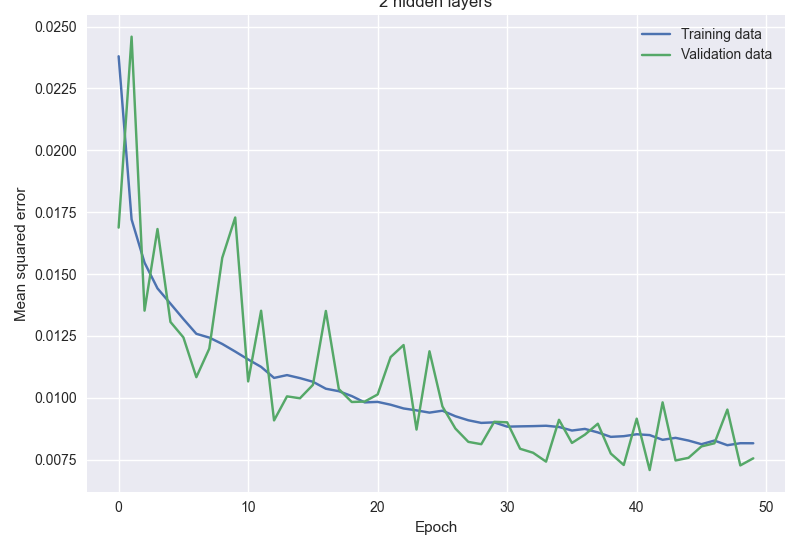
\includegraphics[width=\linewidth]{Figures/test2Layers.png}
\end{subfigure}
\caption{Training and validation data loss function (MSE) over each epoch for the test architecture.}
\label{fig:test}
\end{figure}

While the results are admittedly fairly satisfactory, I would like to try to really use the common tools of NN.
Firstly, instead of using a fixed learning rate, we will use adaptive one using ReduceLROnPlateau function.
To reduce noise in the results, the data will be K-fold Cross-validated, and I will also perform a grid-search CV, changing batch size, number of epochs, number of layers, and ativation functions.

ISTO KOT PREJ ZA NAJBOLJSI MODEL
SLIKA UTEZI ZA NAJBOLJSI MODEL

PRIKAZ NAPAK NA TEST PODATKIH

Finally, we can perform some measures to improve the model's robustness and reduce overfitting. For that reason I have included noisy data in the training set (after all, we expect real life data to be noisy as well), tested some kernel regularizers and dropout neuron method.




\end{document}